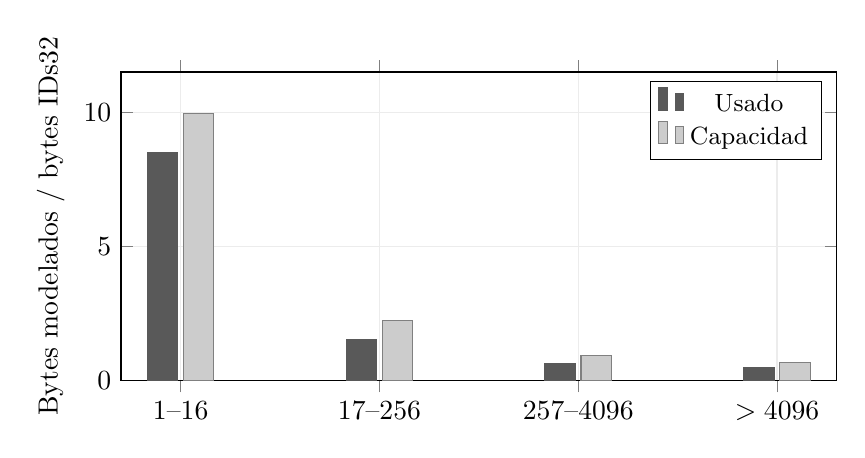
\begin{tikzpicture}
\begin{axis}[ybar,bar width=11pt,width=0.88\textwidth,height=5.5cm,ymin=0,ymax=11.5,
ylabel={Bytes modelados / bytes IDs32},symbolic x coords={a,b,c,d},xtick=data,
xticklabels={1--16,17--256,257--4096,$>4096$},
legend style={at={(0.98,0.97)},anchor=north east,font=\small},grid=major,grid style={gray!15}]
\addplot[fill=black!65,draw=black!65] coordinates {(a,8.496759822) (b,1.519760317) (c,0.622734497) (d,0.479418480)};
\addplot[fill=black!20,draw=black!50] coordinates {(a,9.953422438) (b,2.242846005) (c,0.924031758) (d,0.658488922)};
\legend{Usado,Capacidad}
\end{axis}
\end{tikzpicture}
